\documentclass[10pt,a4paper]{article}

\usepackage[utf8]{inputenc}
\usepackage[T1]{fontenc}
\usepackage[margin=1.65cm]{geometry}
\usepackage{graphicx}
\usepackage{amsmath,amssymb}
\usepackage{caption}
\usepackage{microtype}
\usepackage{tikz}
\usetikzlibrary{positioning,arrows.meta}
\usepackage[colorlinks=true,linkcolor=blue,urlcolor=blue]{hyperref}
\usepackage[UTF8]{ctex}

\graphicspath{{photo/}}
\captionsetup{font=footnotesize,skip=3pt}
\setlength{\parindent}{0pt}
\setlength{\parskip}{3pt}

\title{\vspace{-1.2em}Computer Vision: RC-Car Global Vision\vspace{-0.5em}}
\author{KEVIN 常凱文 \\ \small Computer Vision --- Assignment 1, National Taiwan Normal University}
\date{June 2026}

\begin{document}
\maketitle
\vspace{-1.5em}

\section{Introduction and objective}

The goal is to build a global-vision server for an RC-car playing field.  A
camera is mounted on a selfie stick or tripod at a side angle so that the
whole field is visible.  Image measurements are converted to the real
two-dimensional field coordinate system using camera calibration and a
planar homography.  The required output for each detected car is

\begin{center}
\small
\begin{tabular}{ll}
\textbf{timestamp} & relative time in microseconds\\
\textbf{car ID} & identifier of the detected car\\
\textbf{position} & $(x,y)$ in millimeters, or $(-1000,-1000)$ if absent\\
\textbf{orientation} & $\theta$ in degrees\\
\textbf{velocity} & $(dx,dy)$ in millimeters per second\\
\textbf{angular velocity} & degrees per second\\
\textbf{image position} & $(u,v)$ pixel coordinates of the car center
\end{tabular}
\end{center}

\section{Car detection}

Ultralytics SAM3 detects the RC car with the text prompt
\texttt{toy car}.  For every camera frame, the image is passed to SAM3,
which returns a confidence score, a segmentation mask, and a bounding box.
The pixel center is obtained from the detected box (or mask) and is used as
the image coordinate $(u,v)$.  Comparing consecutive positions and their
timestamps gives image motion; after the homography, the same calculation
gives $(dx,dy)$ in millimeters per second.  The orientation is obtained from
the direction of the car, and the difference between consecutive orientations
gives angular velocity.

\begin{figure}[ht]
\centering
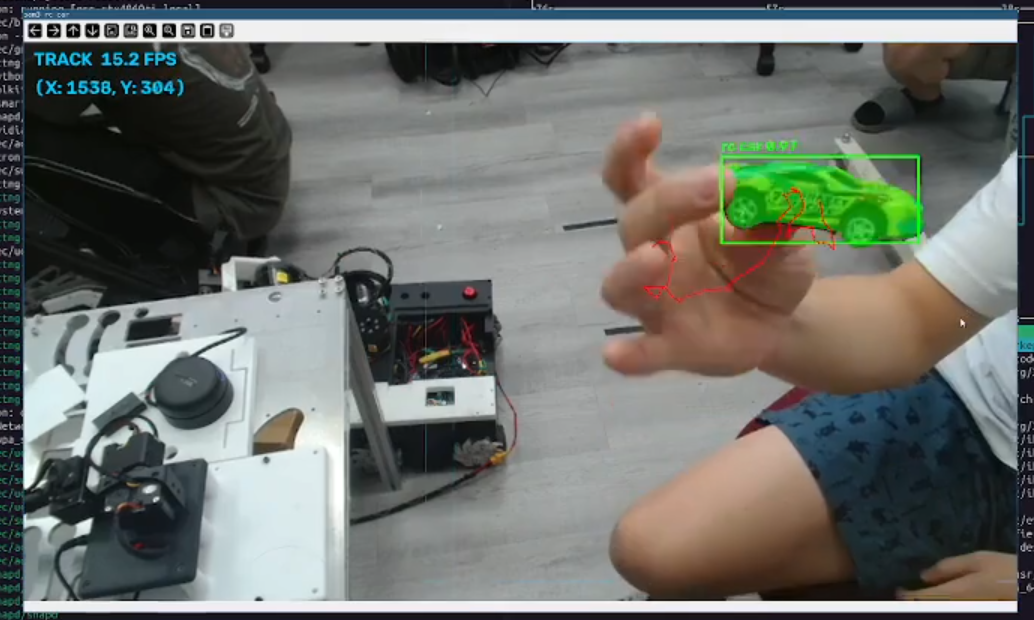
\includegraphics[width=.62\textwidth]{track_car.png}
\caption{SAM3 live result.  The green mask is the segmented car, the
rectangle is its bounding box, and the red points are the tracked center.
The camera frame is \(1920\times1080\); \texttt{imgsz=644} is only the
model's internal inference size.}
\label{fig:sam3}
\end{figure}

\section{Camera calibration}

The lens causes distortion, so pixel coordinates are corrected before
mapping.  A printed Charuco board using \texttt{DICT\_6X6\_250}, 25-mm
squares, and 18-mm markers is observed at different positions and angles.
OpenCV detects the Charuco corners and estimates the camera matrix $K$ and
distortion coefficients with \texttt{cv2.calibrateCamera()}:

\begin{verbatim}
error, K, distortion, rvecs, tvecs =
    cv2.calibrateCamera(object_points, image_points, image_size, ...)
undistorted = cv2.undistort(frame, K, distortion)
\end{verbatim}

\begin{figure}[ht]
\centering
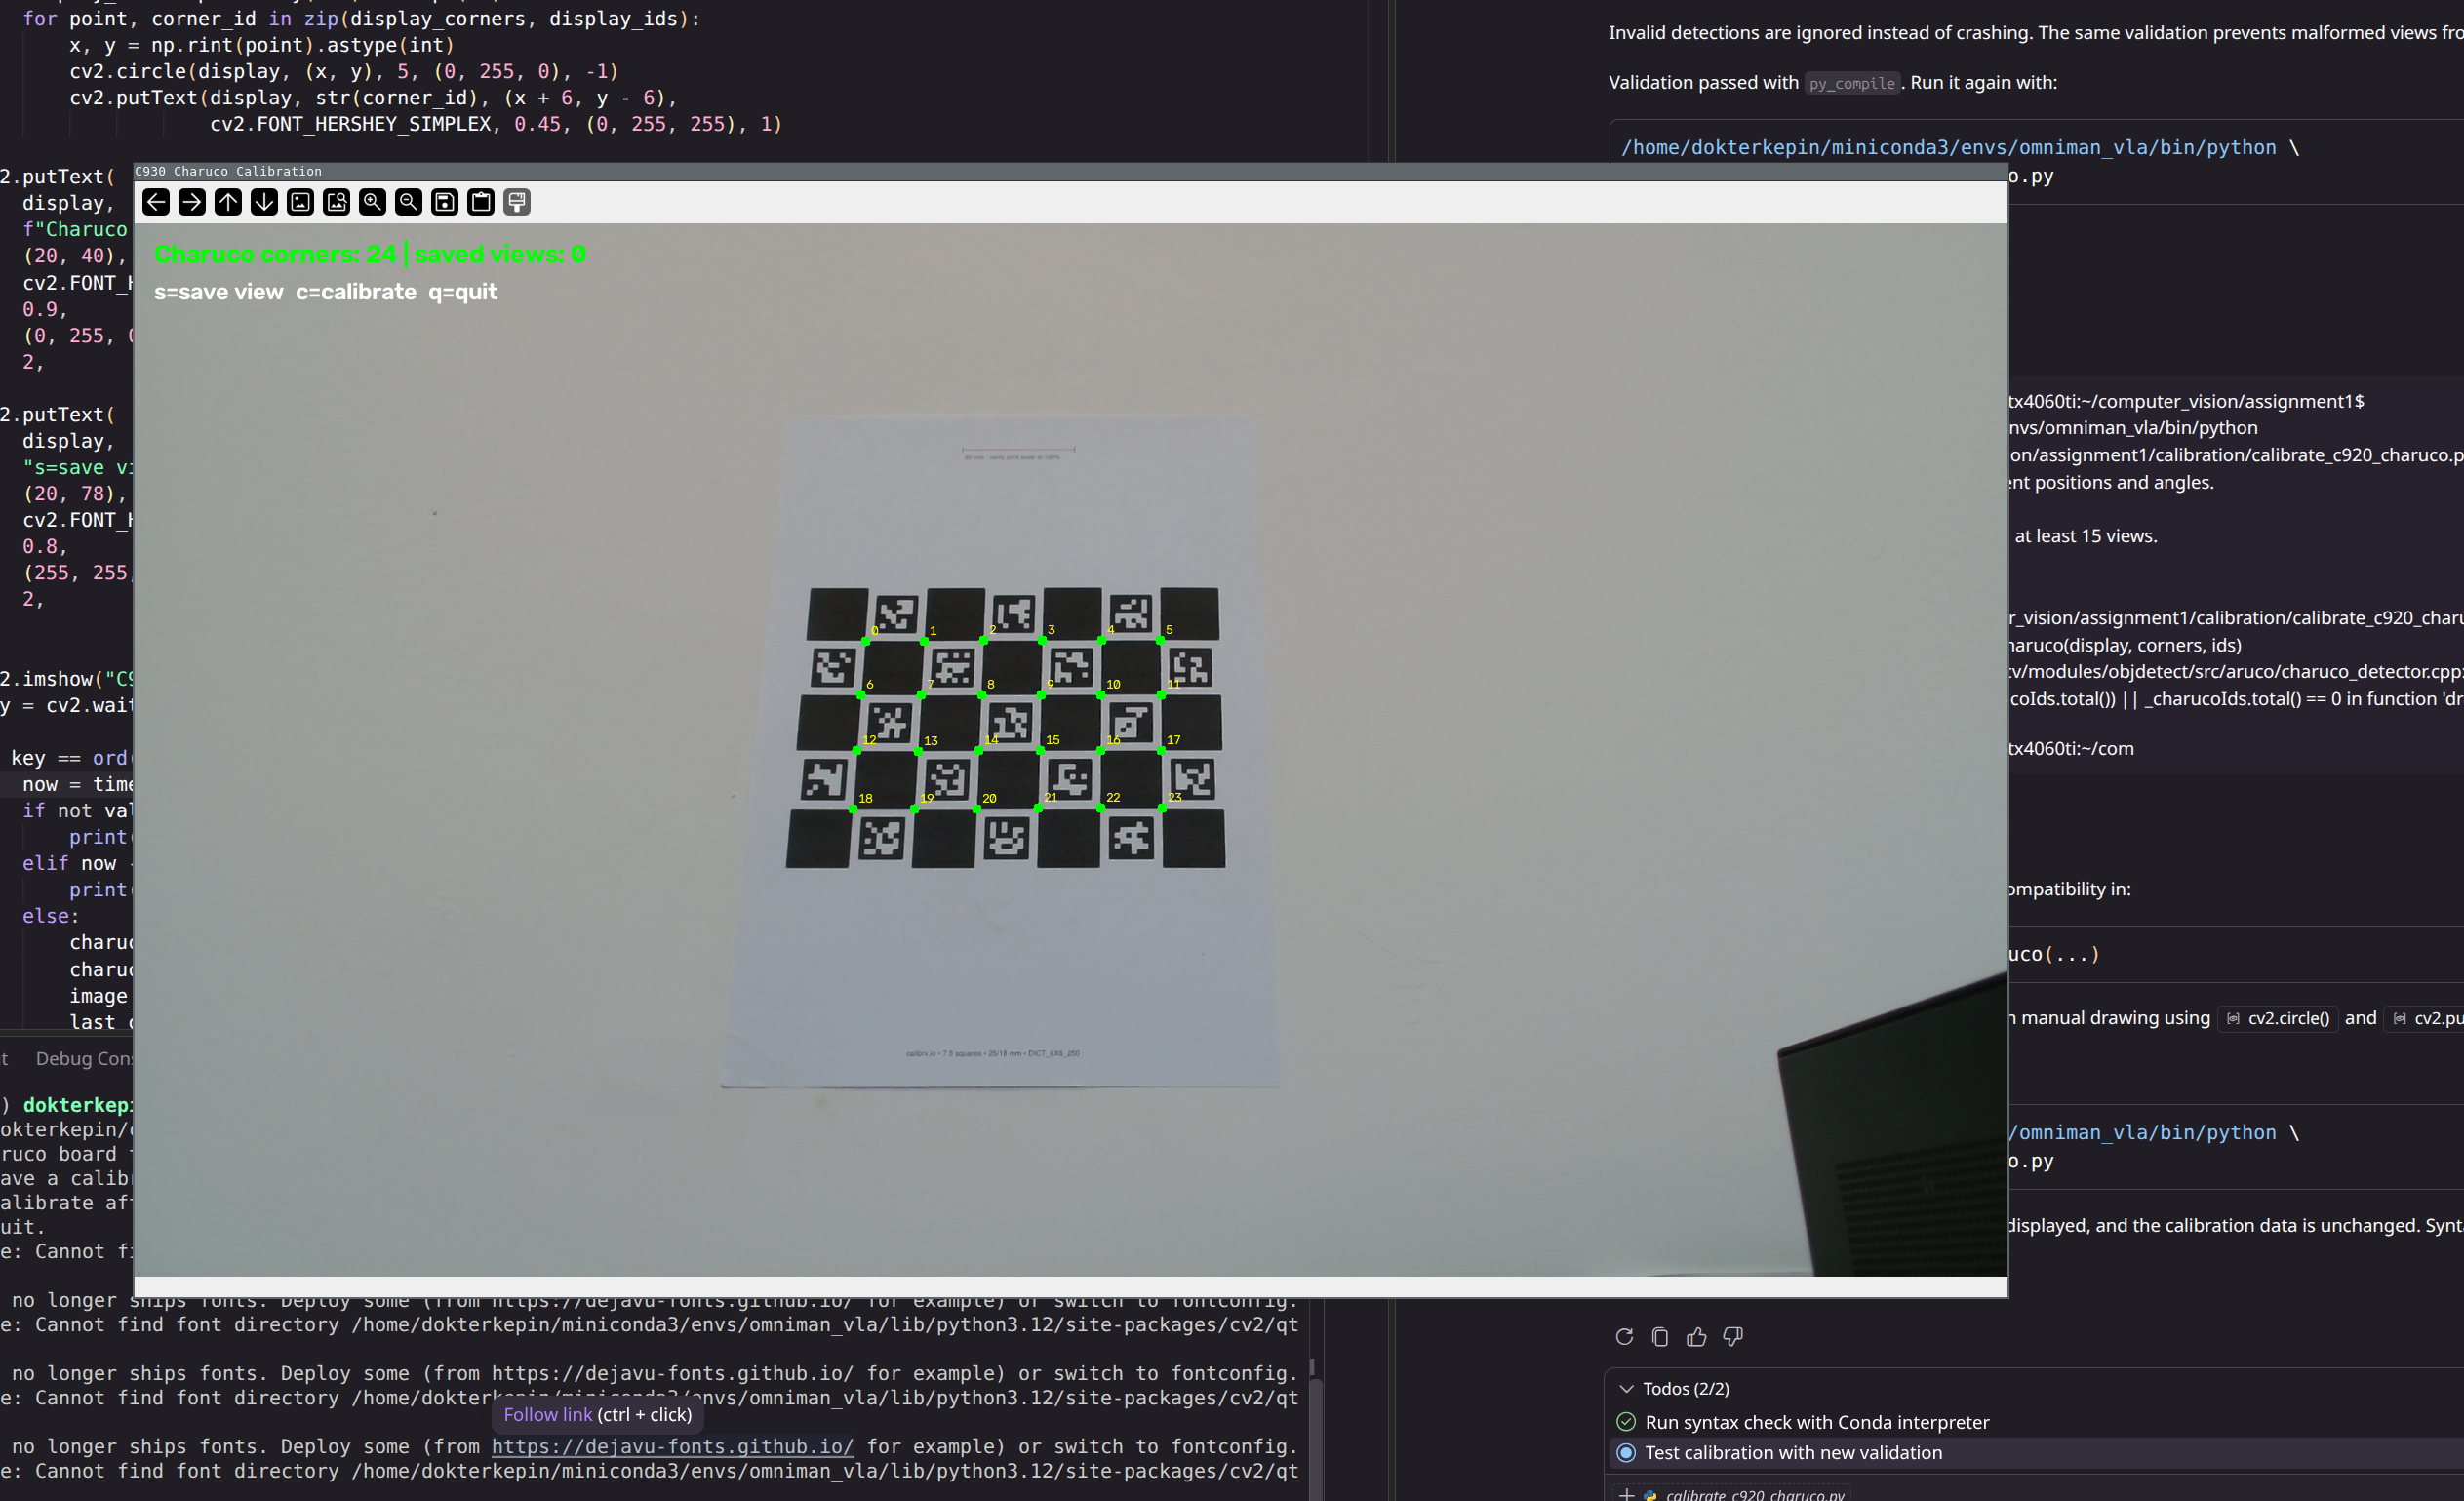
\includegraphics[width=.58\textwidth]{charuco.png}
\caption{Detected Charuco corners (green).  The board supplies known
planar points for estimating lens distortion; it is not used as the field
coordinate frame.  The calibration is saved for the same \(1920\times1080\)
runtime resolution.}
\label{fig:charuco}
\end{figure}

\section{AprilTag field coordinate frame}

Four fixed \texttt{tag36h11} AprilTags outside the playing area define a
known rectangle.  The physical dimensions are measured from tag center to
tag center, not from paper edges:

\begin{center}
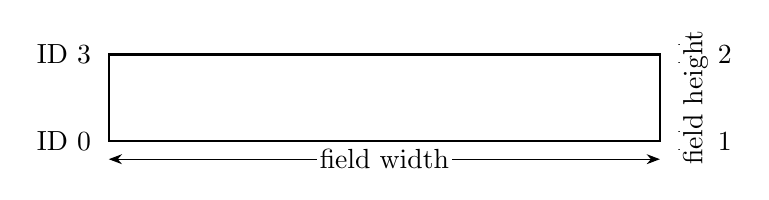
\begin{tikzpicture}[x=1cm,y=0.55cm,>=Stealth]
\draw[thick] (0,0) -- (7,0) -- (7,2) -- (0,2) -- cycle;
\node[anchor=east] at (-.1,0) {ID 0};
\node[anchor=west] at (7.1,0) {ID 1};
\node[anchor=east] at (-.1,2) {ID 3};
\node[anchor=west] at (7.1,2) {ID 2};
\draw[<->] (0,-.42) -- node[fill=white,inner sep=1pt] {\(\text{field width}\)} (7,-.42);
\draw[<->] (7.45,0) -- node[fill=white,inner sep=1pt,rotate=90] {\(\text{field height}\)} (7.45,2);
\end{tikzpicture}
\end{center}

In this arrangement, ID 0 is the origin $(0,0)$, ID 1 is
$(W,0)$, ID 2 is $(W,H)$, and ID 3 is $(0,H)$.  Thus the labels in the
AprilTag photograph mean
\[
\begin{array}{ccc}
\text{ID 3} & \text{--- } W\text{ mm ---} & \text{ID 2}\\[-2pt]
\vert && \vert\\[-2pt]
\text{ID 0} & \text{--- } W\text{ mm ---} & \text{ID 1}
\end{array}
\]
where the vertical separation is $H$ mm.  The drawing is a top view and all
dimensions are between marker centers.  In the measured setup,
$W=280$ mm and $H=340$ mm.

\begin{figure}[ht]
\centering
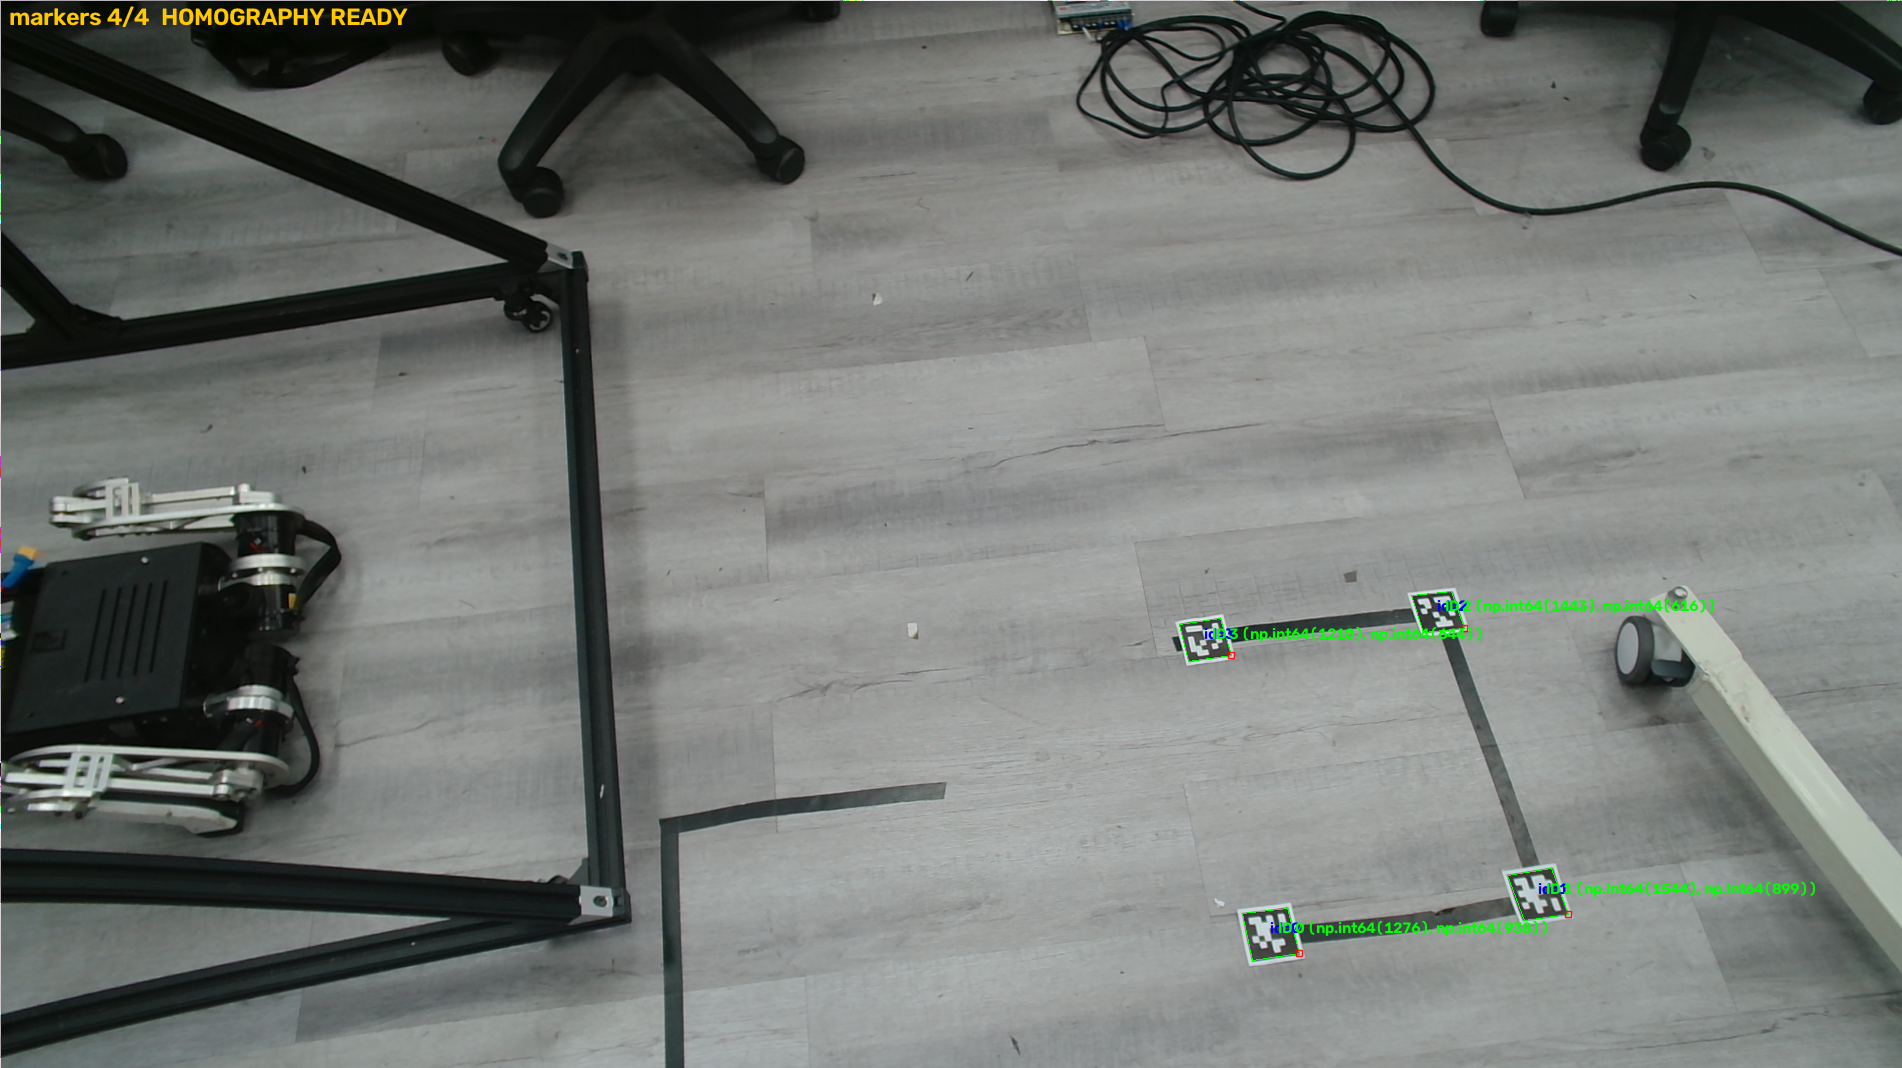
\includegraphics[width=.72\textwidth]{april_tag.png}
\caption{AprilTag field references.  OpenCV detects each tag corner and
computes its center in pixels.  The four centers are paired with the
millimeter coordinates above; the text ``HOMOGRAPHY READY'' means that all
four non-collinear correspondences were found.}
\label{fig:tags}
\end{figure}

\section{Homography and real-world output}

After undistortion, the detected tag centers form image points
$p_i=(u_i,v_i)$ and the measured layout forms world points
$P_i=(x_i,y_i)$.  OpenCV computes the image-to-floor transformation:

\begin{verbatim}
H, _ = cv2.findHomography(image_points, world_points)
floor_point = cv2.perspectiveTransform(pixel_point, H)
\end{verbatim}

The $3\times3$ matrix $H$ maps any point on the floor from pixels to
millimeters.  It corrects perspective, so there is no single
millimeters-per-pixel value across the image.  The bottom-center of the
car detection is used when the desired point is the car's contact with the
floor; the car center is reported according to the assignment convention.
The camera and tags remain fixed while $H$ is used.

\begin{figure}[ht]
\centering
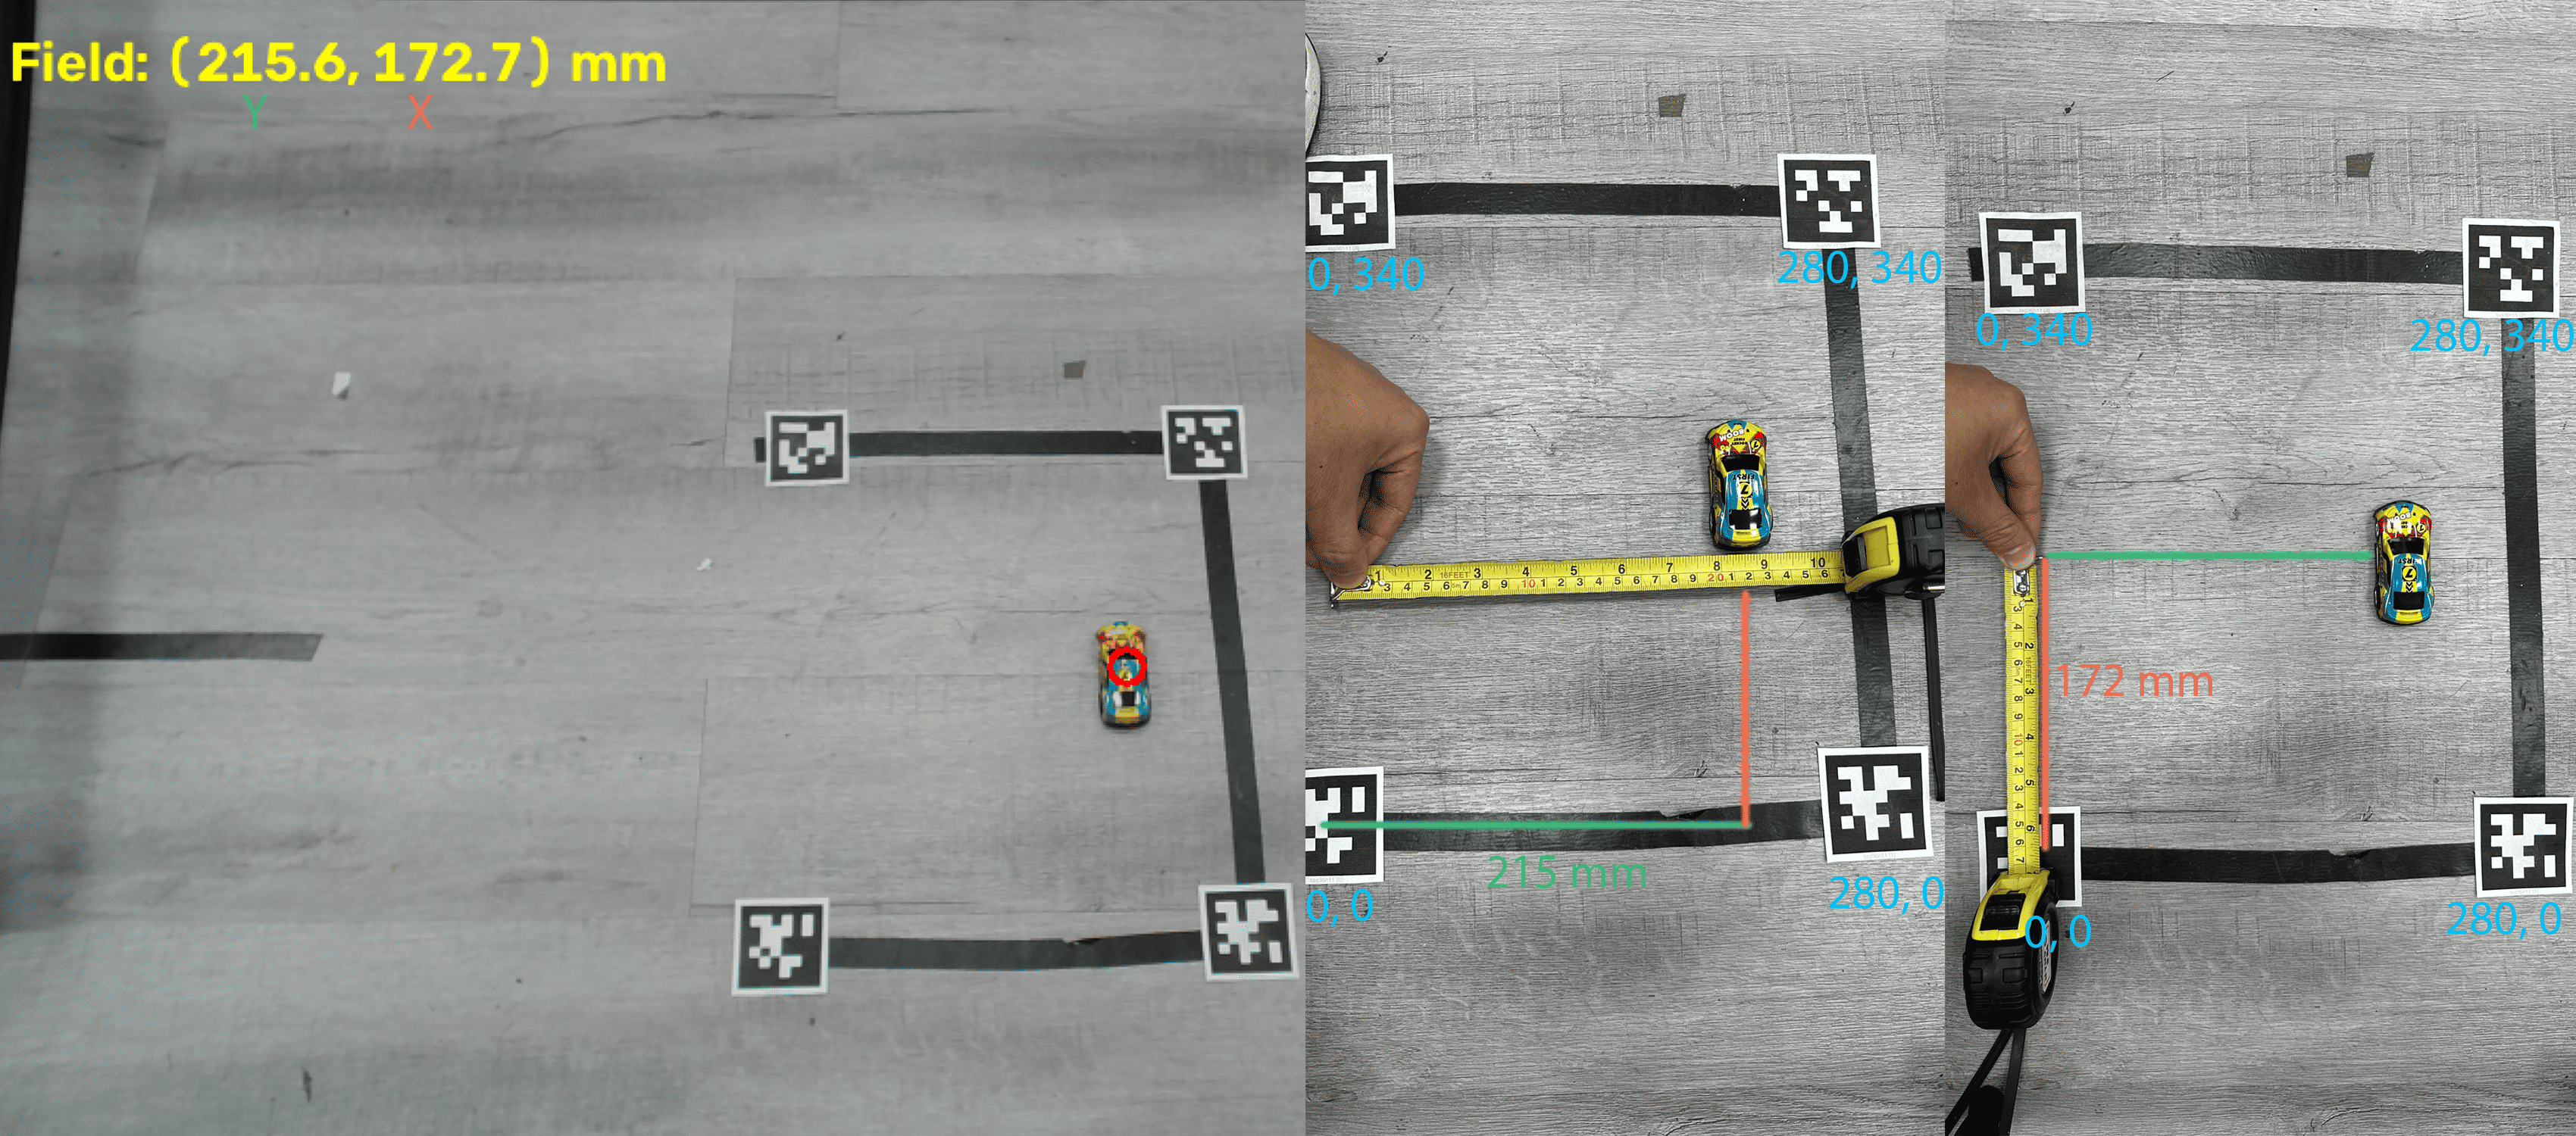
\includegraphics[width=.49\textwidth]{test1_edited.png}\hfill
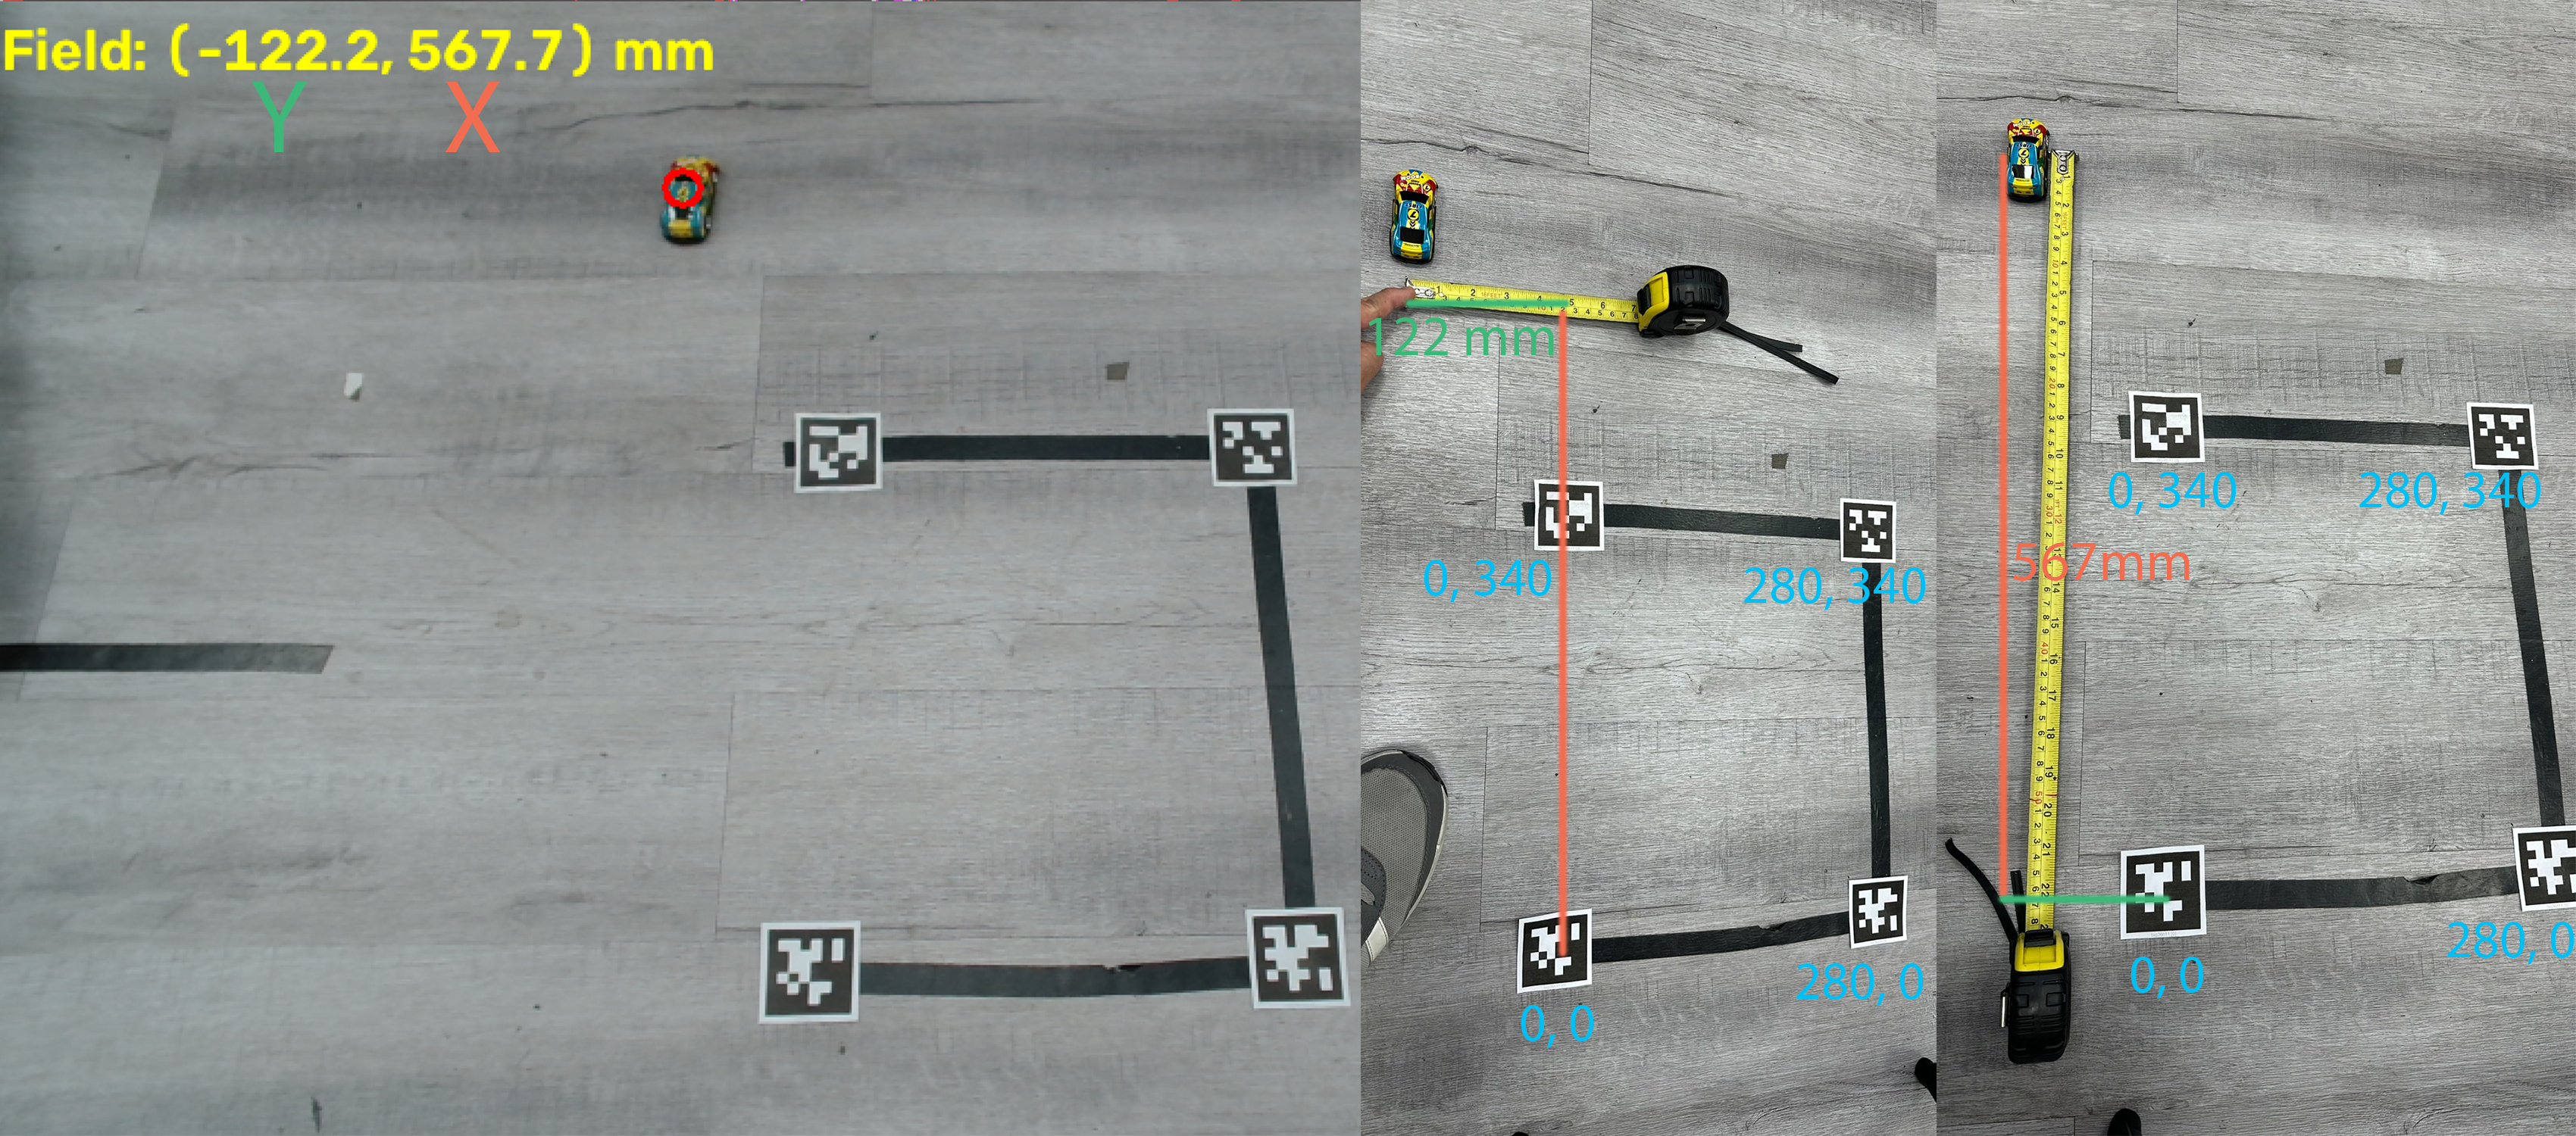
\includegraphics[width=.49\textwidth]{test2_edited.png}
\caption{Metric checks at two car positions.  The annotated ruler readings
are compared with the $(x,y)$ values produced by transforming the detected
image point with $H$.  These checks verify both the tag-center convention
and the millimeter scale.}
\label{fig:checks}
\end{figure}

\section{Complete processing chain}

The server therefore performs the following sequence for each frame:
\textbf{(1)} capture and undistort the image; \textbf{(2)} detect the car
with SAM3 and obtain $(u,v)$; \textbf{(3)} transform the point with $H$ to
obtain $(x,y)$ in millimeters; \textbf{(4)} estimate $\theta$ from the car
direction; and \textbf{(5)} use timestamped consecutive measurements to
calculate linear and angular velocity.  It then publishes the timestamp,
car ID, world position, orientation, velocities, and image coordinates in
the required format.  If no car is detected, the position fields are
$(-1000.0,-1000.0)$.

\end{document}
